% Copyright (c) 2021-10-07 Eclipse Arrowhead Project
%
% This program and the accompanying materials are made available under the
% terms of the Eclipse Public License 2.0 which is available at
% http://www.eclipse.org/legal/epl-2.0.
%
% SPDX-License-Identifier: EPL-2.0

This section is what constitutes the \GlossaryHyperRef{model-reference}{reference model} of this document.
Each of its subsections \GlossaryHyperRef{description}{describes} a primary Arrowhead concept, which are as follows:

\vspace*{0.25cm}
\begin{itemize}[leftmargin=1.2cm,rightmargin=0pt,labelwidth=1cm,labelsep=0pt,itemindent=0pt,parsep=0pt,topsep=0pt,align=left]
\item[\ref{sec:reference-model:stakeholder}] \textbf{\nameref{sec:reference-model:stakeholder}}
\item[\ref{sec:reference-model:entity}] \textbf{\nameref{sec:reference-model:entity}}
\item[\ref{sec:reference-model:device}] \textbf{\nameref{sec:reference-model:device}}
\item[\ref{sec:reference-model:system}] \textbf{\nameref{sec:reference-model:system}}
\item[\ref{sec:reference-model:service}] \textbf{\nameref{sec:reference-model:service}}
\item[\ref{sec:reference-model:system-of-systems}] \textbf{\nameref{sec:reference-model:system-of-systems}}
\vspace*{0.1cm}
\begin{itemize}[leftmargin=1cm,rightmargin=0pt,labelwidth=1cm,labelsep=0pt,itemindent=0pt,parsep=0.05cm,topsep=0.05cm,align=left]
  \item[\ref{sec:reference-model:system-of-systems:local-cloud}] \textbf{\nameref{sec:reference-model:system-of-systems:local-cloud}}
  \item[\ref{sec:reference-model:system-of-systems:system-of-local-clouds}] \textbf{\nameref{sec:reference-model:system-of-systems:system-of-local-clouds}}
\end{itemize}
\vspace*{0.1cm}
\item[\ref{sec:reference-model:network}] \textbf{\nameref{sec:reference-model:network}}
\item[\ref{sec:reference-model:interface}] \textbf{\nameref{sec:reference-model:interface}}
\item[\ref{sec:reference-model:policy}] \textbf{\nameref{sec:reference-model:policy}}
\item[\ref{sec:reference-model:protocol}] \textbf{\nameref{sec:reference-model:protocol}}
\item[\ref{sec:reference-model:data}] \textbf{\nameref{sec:reference-model:data}}
\end{itemize}
\vspace*{0.25cm}

\subsection{Stakeholder}
\label{sec:reference-model:stakeholder}

A \GlossaryHyperRef{stakeholder}{stakeholder} is a person or \GlossaryHyperRef{organization}{organization} with stake in an \GlossaryHyperRef{entity}{entity} or undertaking with relevance to the \GlossaryHyperRef{framework-arrowhead}{Arrowhead framework}.
In this context, we understand \GlossaryHyperRef{stake}{\textit{stake}} to refer to any type of engagement or commitment.
The concept is illustrated in Figure \ref{fig:stakeholder}, which also lists five reasons why a given person or organization is to be considered a stakeholder.
We refer to these reasons as \GlossaryHyperRef{role-stakeholder}{\textit{roles}}.

\begin{figure}[ht!]
  \centering
  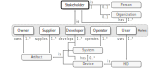
\includegraphics{figures/stakeholder}
  \caption{
    The stakeholder as either a person or organization, where each such stakeholder takes on one ore more distinct roles.
    \GlossaryHyperRef{hid}{HID} is an abbreviation for \GlossaryHyperRef{device-human-interface}{Human Interface Device}.
  }
  \label{fig:stakeholder}
\end{figure}

The roles occupied by a given stakeholder dictates what \GlossaryHyperRef{entity}{entities} that person or organization will interact with, as well as the nature of that interaction.
In Figure \ref{fig:stakeholder}, (1) \GlossaryHyperRef{owner}{owner}, (2) \GlossaryHyperRef{designer}{designer}, (3) \GlossaryHyperRef{developer}{developer}, (4) \GlossaryHyperRef{operator}{operator} and (5) \GlossaryHyperRef{user}{user} are named explicitly, but more roles are likely to be relevant.
Use of the listed names is preferred over any synonyms when referring to these particular roles.
Refer to the \hyperref[sec:glossary]{glossary} for their definitions.

\subsection{Entity}
\label{sec:reference-model:entity}

\begin{figure}[ht!]
  \centering
  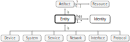
\includegraphics{figures/entity}
  \caption{
    X
  }
  \label{fig:entity}
\end{figure}

\subsection{Device}
\label{sec:reference-model:device}

\begin{figure}[ht!]
  \centering
  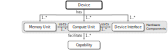
\includegraphics{figures/device}
  \caption{
    X
  }
  \label{fig:device}
\end{figure}

\subsection{System}
\label{sec:reference-model:system}

\begin{figure}[ht!]
  \centering
  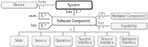
\includegraphics{figures/system}
  \caption{
    X
  }
  \label{fig:system}
\end{figure}

The system has its own identity. A single software artifact can host multiple systems, given that each system is distinct from all others.

\subsection{Service}
\label{sec:reference-model:service}

\begin{figure}[ht!]
  \centering
  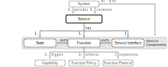
\includegraphics{figures/service}
  \caption{
    X
  }
  \label{fig:service}
\end{figure}

TODO: Explain function invocation. Separate diagram?

\subsection{System-of-Systems}
\label{sec:reference-model:system-of-systems}

\begin{figure}[ht!]
  \centering
  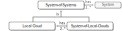
\includegraphics{figures/system-of-systems}
  \caption{
    X
  }
  \label{fig:system-of-systems}
\end{figure}

\subsubsection{Local Cloud}
\label{sec:reference-model:system-of-systems:local-cloud}

\begin{figure}[ht!]
  \centering
  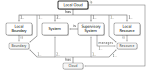
\includegraphics{figures/local-cloud}
  \caption{
    X
  }
  \label{fig:local-cloud}
\end{figure}

\subsubsection{System-of-Local-Clouds}
\label{sec:reference-model:system-of-systems:system-of-local-clouds}

X

\subsection{Network}
\label{sec:reference-model:network}

\begin{figure}[ht!]
  \centering
  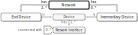
\includegraphics{figures/network}
  \caption{
    X
  }
  \label{fig:network}
\end{figure}

\subsection{Interface}
\label{sec:reference-model:interface}

\begin{figure}[ht!]
  \centering
  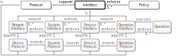
\includegraphics{figures/interface}
  \caption{
    X
  }
  \label{fig:interface}
\end{figure}

TODO: Discussion about difference between interface and service?

\subsection{Policy}
\label{sec:reference-model:policy}

\begin{figure}[ht!]
  \centering
  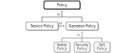
\includegraphics{figures/policy}
  \caption{
    X
  }
  \label{fig:policy}
\end{figure}

\subsection{Protocol}
\label{sec:reference-model:protocol}

\begin{figure}[ht!]
  \centering
  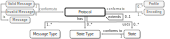
\includegraphics{figures/protocol}
  \caption{
    X
  }
  \label{fig:protocol}
\end{figure}


\subsection{Data}
\label{sec:reference-model:data}

\begin{figure}[ht!]
  \centering
  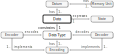
\includegraphics{figures/data}
  \caption{
    X
  }
  \label{fig:data}
\end{figure}